\section{Introduzione alla Gestione delle Identità e degli Accessi}
La gestione delle identità e degli accessi (IAM) rappresenta, a mio avviso, il fondamento di qualsiasi strategia di sicurezza robusta in un ambiente cloud come Amazon Web Services (AWS). Per una startup fintech, dove la protezione dei dati sensibili e la continuità operativa sono vitali, definire chi può accedere a cosa e con quali privilegi non è solo una best practice, ma una necessità imprescindibile. Questo capitolo esplora i principi cardine della sicurezza IAM, analizza la configurazione attuale della startup "Finanz" e propone una serie di miglioramenti concreti per rafforzare la postura di sicurezza, ispirandosi ai modelli Zero Trust e al Principio del Minimo Privilegio. L'obiettivo è creare un framework IAM che sia non solo sicuro, ma anche flessibile e gestibile, per supportare la crescita dinamica della startup.

\section{Principi di Sicurezza per la Gestione delle Identità e degli Accessi e Analisi del Contesto Attuale}
\label{sec:principi-identita-accessi}
\section{Configurazione Attuale dell'Ambiente AWS di Finanz (Focus Infrastrutturale)}
\label{sec:aws_infrastruttura_attuale_cap2}
Prima di addentrarci nelle specifiche di sicurezza, è utile richiamare brevemente la configurazione infrastrutturale di Finanz, focalizzandoci sugli aspetti non prettamente IAM, già trattati.
L'infrastruttura cloud della startup è stata realizzata utilizzando i servizi di Amazon Web Services (AWS), con le operazioni principali concentrate nella regione geografica \texttt{eu-south-1} (Milano). Come già menzionato, l'account AWS (\texttt{478291635847}) è configurato con una separazione degli ambienti: \texttt{Finanz-Dev} per lo sviluppo e \texttt{Finanz-Prod} per l'applicazione in uso dagli utenti finali.

Il cuore dell'infrastruttura applicativa è \textbf{AWS Elastic Beanstalk}. Questo servizio semplifica il rilascio e la gestione delle applicazioni "Finanz". L'ambiente di sviluppo utilizza la configurazione \texttt{finanz-dev-v2} mentre quello di produzione opera su \texttt{finanz-prod-v1.3}. Elastic Beanstalk orchestra la creazione e configurazione delle risorse necessarie, come le macchine virtuali \textbf{Amazon EC2}. Per queste, ho osservato l'uso di istanze di tipo \texttt{t3a.small} per lo sviluppo e \texttt{t3a.medium} per la produzione, scelte per il loro buon rapporto prezzo-prestazioni per carichi di lavoro di piccole e medie dimensioni. Tipicamente, l'ambiente di sviluppo gestisce 1-2 istanze, mentre quello di produzione ne mantiene attive 3-5, scalando automaticamente durante i picchi di utilizzo grazie all'auto-scaling gestito da Elastic Beanstalk. Per l'ambiente di produzione, un \textbf{Application Load Balancer (ALB)} denominato \texttt{finanz-prod-alb-1284567} distribuisce le richieste degli utenti alle istanze EC2.

Per la gestione dei dati, Finanz utilizza \textbf{Amazon RDS for PostgreSQL}. Ho constatato la presenza di due istanze database separate: una per lo sviluppo (\texttt{finanz-dev-db.cluster-cx4s7k9m2qla.eu-south-1.rds.amazonaws.com}, di tipo \texttt{db.t4g.micro}) e una per la produzione (\texttt{finanz-prod-db.cluster-cx4s7k9m2qlb.eu-south-1.rds.amazonaws.com}, di tipo \texttt{db.t4g.small}). L'istanza di sviluppo gestisce circa 50-100 connessioni simultanee con un database di circa 2GB, mentre quella di produzione arriva a gestire fino a 500 connessioni con un database di circa 15GB. L'istanza di produzione è configurata in modalità \textbf{Multi-AZ} (Multi-Availability Zone) e entrambe le istanze RDS sono protette da crittografia a riposo, con chiavi gestite dal servizio \textbf{AWS KMS} (la chiave specifica per RDS è \texttt{arn:aws:kms:eu-south-1:478291635847:key/12345678-1234-1234-1234-123456789012}, come menzionato, ma la gestione delle policy di accesso a questa chiave è stata discussa nel capitolo precedente).

La rete virtuale privata della startup è definita tramite \textbf{Amazon VPC (Virtual Private Cloud)}, chiamato "Finanz-vpc" con CIDR block \texttt{10.0.0.0/16}. All'interno di questo VPC, lo spazio di indirizzi IP è diviso in \textbf{subnet} pubbliche (\texttt{10.0.1.0/24}, \texttt{10.0.2.0/24}) e private (\texttt{10.0.10.0/24}, \texttt{10.0.11.0/24}, \texttt{10.0.12.0/24}), distribuite su diverse \textbf{Availability Zones} (\texttt{eu-south-1a}, \texttt{eu-south-1b}, \texttt{eu-south-1c}). La connettività verso Internet è fornita da un \textbf{Internet Gateway} (\texttt{igw-0a1b2c3d4e5f67890}) e un \textbf{VPC Endpoint per S3} (\texttt{vpce-1a2b3c4d5e6f7g8h9}) permette la comunicazione privata con S3.

\textbf{Amazon S3 (Simple Storage Service)} è utilizzato per:
\begin{itemize}
    \item Archiviazione dei file di log (bucket \texttt{finanz-logs-478291635847}).
    \item Salvataggio degli artefatti di build da \textbf{AWS CodePipeline} (bucket \texttt{finanz-artifacts-eu-south-1}).
    \item Hosting di file statici per le applicazioni web (bucket \texttt{finanz-static-assets}), serviti tramite una distribuzione CloudFront (\texttt{E1A2B3C4D5E6F7}).
\end{itemize}
La crittografia lato server con chiavi KMS e l'imposizione di HTTPS sono pratiche già in uso per S3.

Infine, per l'automazione del rilascio software, Finanz si avvale di \textbf{AWS CodePipeline} e \textbf{AWS CodeBuild}, con notifiche gestite da \textbf{AWS SNS (Simple Notification Service)}.

\begin{figure}[h]
  \centering
  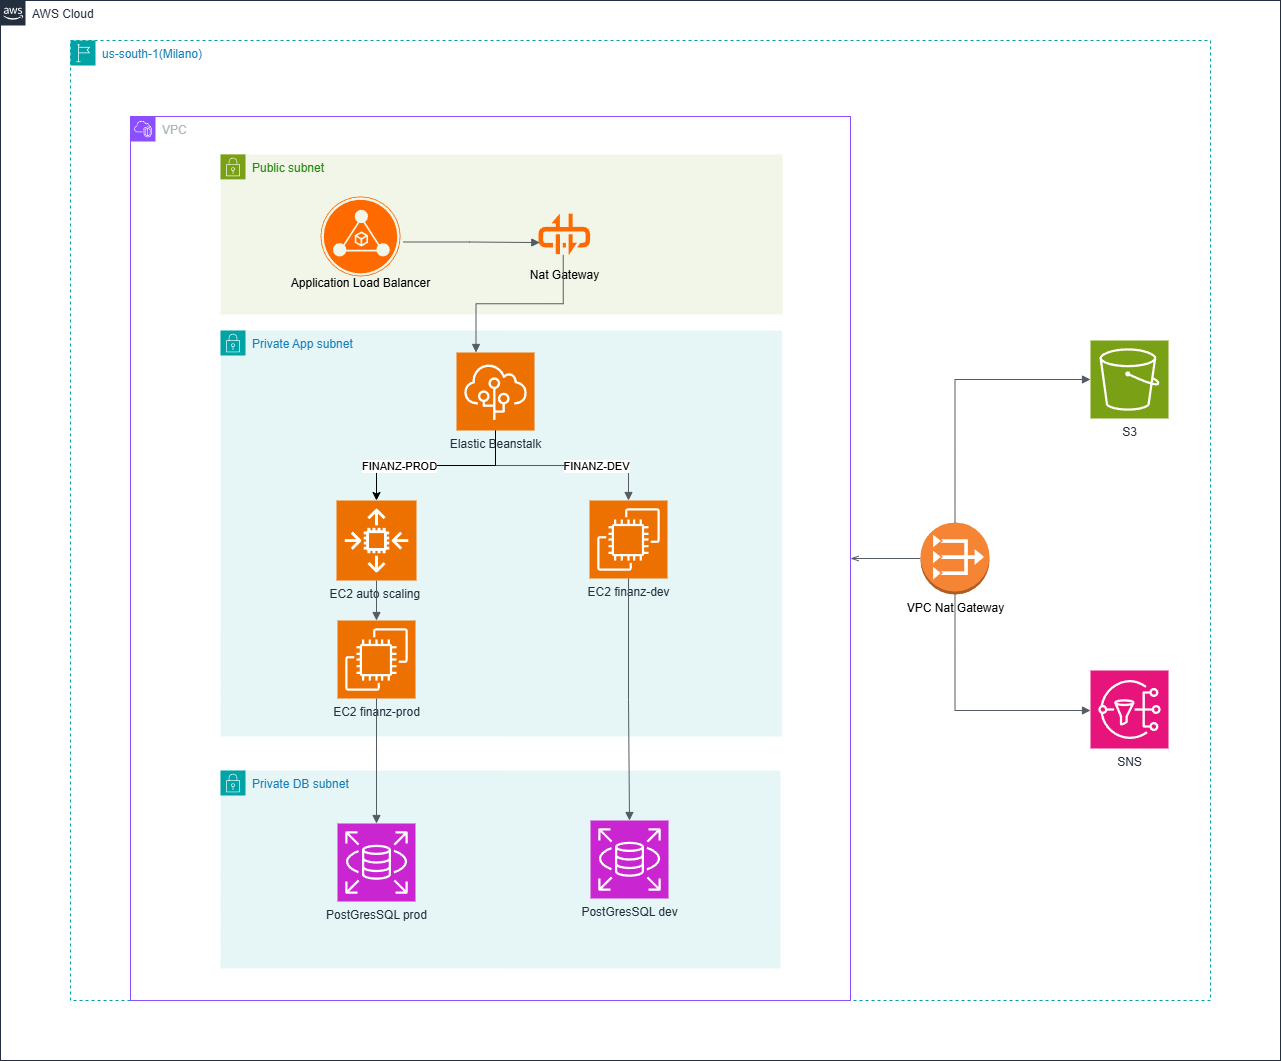
\includegraphics[width=0.8\textwidth]{aws_struttura} % Assicurati che il file 'aws_struttura.png' o simile sia nella stessa cartella o in un percorso specificato
  \caption{Diagramma semplificato dell'architettura attuale di Finanz in AWS.}
  \label{fig:aws_struttura_attuale_cap2}
\end{figure}

\subsection{Implementazione del Modello Zero Trust e del Principio del Minimo Privilegio}
\label{sec:zero-trust-implementation}

Come ho avuto modo di approfondire precedentemente [NdR: qui potresti riferirti a un capitolo teorico precedente, se esiste, con `\ref{ch:principi-cybersecurity}`], il modello \textbf{Zero Trust} rappresenta un cambiamento paradigmatico rispetto alla sicurezza tradizionale basata sul perimetro. Anziché assumere fiducia implicita per le entità all'interno della rete aziendale, il principio cardine è "non fidarsi mai, verificare sempre" (\textit{never trust, always verify}). Ogni richiesta di accesso a una risorsa, indipendentemente dalla sua origine, deve essere esplicitamente autenticata, autorizzata e monitorata. Questo approccio mira a minimizzare la superficie d'attacco e a contenere l'impatto di eventuali compromissioni, risultando particolarmente critico per proteggere la \textit{business continuity} aziendale. Ritengo che l'adozione di questo principio sia particolarmente rilevante nel contesto delle startup, caratterizzate da ambienti operativi dinamici e altamente flessibili. Le startup presentano peculiarità che amplificano l'esigenza di un solido framework di sicurezza:

\begin{itemize}
    \item \textbf{Instabilità relazionale:} Le relazioni professionali nelle startup possono deteriorarsi rapidamente, sia a livello dirigenziale che operativo. Secondo un'analisi di CB Insights, i conflitti interni tra fondatori rappresentano una delle principali cause di fallimento delle startup, incidendo per circa il 13\% dei casi esaminati \cite{CBInsights2023}. 
    \item \textbf{Rischio di attacchi interni:} La fragilità dei rapporti aumenta la probabilità di attacchi da parte di ex-collaboratori con intenti vendicativi. Secondo il "2023 Data Breach Investigations Report" di Verizon, circa il 20\% delle violazioni di dati coinvolge insider con accessi privilegiati \cite{Verizon2023}.
    \item \textbf{Infrastrutture di sicurezza inadeguate:} Le startup, per limitazioni di risorse e focus prevalente sullo sviluppo del prodotto, spesso non dispongono di infrastrutture di sicurezza robuste. Un rapporto di Ponemon Institute evidenzia che le piccole organizzazioni hanno una probabilità tre volte maggiore di subire attacchi informatici rispetto alle grandi imprese, proprio a causa di investimenti insufficienti in sicurezza \cite{Ponemon2023}.
\end{itemize}
Questa sezione illustra come i principi Zero Trust possano essere tradotti in misure di sicurezza concrete all'interno dell'infrastruttura cloud di una startup, con specifico riferimento all'ambiente AWS. Ci concentreremo in particolare sulla gestione delle identità e degli accessi, un pilastro fondamentale per qualsiasi architettura Zero Trust, e sulla sua stretta interconnessione con il \textbf{Principio del Minimo Privilegio (Principle of Least Privilege - PoLP)}.
\subsubsection{Sinergia tra Principio del Minimo Privilegio (PoLP) e Zero Trust}
\label{subsubsec:polp-zerotrust-correlation}

Il Principio del Minimo Privilegio non è solo una buona pratica di sicurezza a sé stante, ma è intrinsecamente legato e \textbf{fondamentale per il successo di un'architettura Zero Trust}. La loro sinergia si manifesta in diversi modi:

\begin{itemize}
    \item \textbf{Riduzione della Superficie d'Attacco:} Limitando strettamente le azioni consentite a ciascuna identità, PoLP riduce l'insieme delle operazioni che un attaccante potrebbe eseguire anche riuscendo a compromettere le credenziali di quell'identità. La verifica dell'identità (Zero Trust) è necessaria ma non sufficiente; i privilegi limitati (PoLP) ne circoscrivono le capacità.
    \item \textbf{Limitazione del Raggio d'Esplosione (\textit{Blast Radius})}: In caso di compromissione o errore, i danni potenziali sono confinati. Un utente o servizio con privilegi minimi non può accedere o modificare risorse al di fuori del suo ambito operativo ristretto, limitando il movimento laterale dell'attaccante e l'impatto dell'incidente.
    \item \textbf{Applicazione della Verifica Esplicita:} Implementare PoLP costringe a definire policy di accesso granulari e intenzionali, basate sulle reali necessità operative. Questo si allinea perfettamente con la richiesta di Zero Trust di basare ogni decisione di accesso su policy esplicite e dinamiche, piuttosto che su autorizzazioni ampie o ereditate implicitamente.
    \item \textbf{Miglioramento del Controllo e dell'Auditabilità:} Policy di accesso minimali e specifiche sono più facili da comprendere, gestire e verificare. Ciò semplifica l'audit della postura di sicurezza e la dimostrazione della conformità, permettendo di attestare che gli accessi sono effettivamente limitati come richiesto dal modello Zero Trust.
\end{itemize}
\subsection{Gestione delle Identità e degli Accessi (IAM) come Pilastro di Zero Trust in AWS}
\label{subsec:iam-zero-trust}

L'infrastruttura ospitata su un Cloud Service Provider (CSP) come AWS è un asset critico per una startup fintech. Essa contiene dati sensibili degli utenti e ospita i servizi essenziali (endpoint API, istanze EC2 per server applicativi, networking VPC, ecc.) che ne garantiscono l'operatività. La protezione di queste risorse inizia dalla gestione rigorosa di chi può accedervi e cosa può fare. \textbf{AWS Identity and Access Management (IAM)} è il servizio centrale per implementare questi controlli e costituisce una base imprescindibile per un modello Zero Trust.

Una delle prime e più critiche aree di intervento riguarda l'\textbf{account root di AWS}. Questo account possiede privilegi illimitati sull'intero ambiente AWS e rappresenta, di conseguenza, un obiettivo di altissimo valore per gli attaccanti e una fonte significativa di rischio operativo se usato impropriamente. Un'implementazione Zero Trust richiede misure stringenti per l'account root:
\begin{itemize}
    \item \textbf{Limitazione Estrema dell'Uso:} L'accesso come utente root deve essere evitato per le operazioni quotidiane e riservato esclusivamente a quelle poche attività che lo richiedono obbligatoriamente (es. modifica delle informazioni di fatturazione, chiusura dell'account, modifica dei piani di supporto).
    \item \textbf{Protezione Robusta delle Credenziali:} La password deve essere estremamente complessa e, soprattutto, l'\textbf{Autenticazione a Più Fattori (MFA)} deve essere \textit{sempre} abilitata e richiesta per l'accesso root.
    \item \textbf{Monitoraggio Continuo:} Ogni azione eseguita tramite l'account root deve essere tracciata e monitorata tramite servizi come AWS CloudTrail, generando allarmi per qualsiasi utilizzo.
\end{itemize}

Per le attività amministrative e operative ordinarie, il modello Zero Trust impone l'utilizzo di \textbf{utenti e ruoli IAM} configurati secondo il \textbf{Principio del Minimo Privilegio (PoLP)}. Come descritto in precedenza [NdR: vedi `\ref{subsubsec:polp-zerotrust-correlation}` o il riferimento a un capitolo teorico], questo principio stabilisce che a un'entità (utente, servizio, applicazione) debbano essere concesse \textit{esclusivamente} le autorizzazioni minime indispensabili per svolgere le proprie funzioni legittime, e non un permesso di più. Ad esempio, un'applicazione che necessita solo di leggere oggetti da un bucket S3 dovrebbe avere un ruolo IAM con solo il permesso `s3:GetObject` su quel bucket specifico, invece di permessi generici su S3 o, peggio, permessi amministrativi.

\subsection{Analisi dell'attuale implementazione di IAM in "Finanz"}
Dall'analisi che ho condotto sull'account AWS della startup Finanz (ID \texttt{478291635847}), sono emerse alcune configurazioni che necessitano di attenzione.

\subsubsection{Configurazione degli Utenti e Ruoli}
L'analisi della struttura IAM esistente rivela la presenza di tre utenti principali: \textbf{Andrea Pasini} (CTO), \textbf{Andrea Ferraboli}, e \textbf{Matteo Giuntoni}. Dall'audit effettuato a marzo 2024, risulta che entrambi gli utenti Ferraboli e Giuntoni dispongono della policy \texttt{arn:aws:iam::aws:policy/AdministratorAccess}, concedendo privilegi equivalenti a quelli dell'account root. L'utente Pasini (User ARN: \texttt{arn:aws:iam::478291635847:user/andrea.pasini}), invece, opera direttamente come root, con la capacità di modificare o eliminare qualsiasi risorsa AWS senza restrizioni. Durante la mia analisi dei log di CloudTrail degli ultimi 3 mesi, ho identificato che l'utente root è stato utilizzato 76 volte, principalmente per operazioni che avrebbero potuto essere delegate a utenti IAM con privilegi più limitati.

Un esame dettagliato delle policy associate mostra l'assenza di \textbf{condizioni contestuali} (es. limitazioni geografiche o orarie) e l'utilizzo esclusivo di policy gestite da AWS, senza personalizzazioni per ridurre i permessi alle effettive necessità operative\cite{ref6}. Ad esempio, l'utente `finanz-backend` (che immagino sia un utente di servizio o un ruolo per un'applicazione) possiede `AmazonS3FullAccess`, sebbene le sue funzioni richiedano solo operazioni di lettura su bucket specifici.

\subsubsection{Criticità Identificate}
Sulla base dell'analisi, ho identificato le seguenti criticità:
\begin{enumerate}
    \item \textbf{Account Root Non Adeguatamente Protetto}: L'account root non utilizza MFA hardware, affidandosi esclusivamente a credenziali statiche (password)\cite{ref3}. Questo lo espone a rischi significativi di compromissione tramite tecniche come phishing o credential stuffing.
    \item \textbf{Privilegi Eccessivi per Utenti IAM}: L'assegnazione indiscriminata della policy `AdministratorAccess` a utenti non root crea superfici di attacco ridondanti. Qualsiasi compromissione di questi account avrebbe un impatto devastante. Inoltre, l'utilizzo diretto dell'account root da parte dell'utente Pasini bypassa qualsiasi meccanismo di controllo basato su policy IAM specifiche\cite{ref2}.
    \item \textbf{Mancanza di Meccanismi di Emergenza}: Non ho riscontrato la presenza di account "break glass" dedicati, essenziali per il ripristino dell'accesso in scenari di compromissione dell'Identity Provider (IdP) o in caso di lockout accidentale degli amministratori\cite{ref4}.
    \item \textbf{Assenza di Monitoring Granulare sulle Azioni IAM}: Sebbene CloudTrail sia attivo, le policy IAM non sembrano integrare logiche di auditing proattivo o condizioni che facilitino il monitoraggio in tempo reale per azioni particolarmente critiche eseguite da specifici utenti o ruoli (es. modifiche a policy IAM stesse, eliminazione di risorse chiave)\cite{ref7}.
\end{enumerate}

\subsubsection{Violazioni delle Best Practice AWS}
L'implementazione corrente, a mio parere, non è allineata con alcune raccomandazioni fondamentali del framework \textbf{AWS Foundational Security Best Practices}:
\begin{itemize}
    \item \textbf{FSBP IAM-1}: Mancanza di MFA hardware per l'utente root\cite{ref3}.
    \item \textbf{FSBP IAM-7}: Assegnazione di policy con privilegi non limitati al minimo necessario per svolgere le funzioni richieste\cite{ref5}.
    \item \textbf{FSBP IAM-8}: Mancanza di un chiaro allineamento tra i ruoli IAM definiti e le responsabilità organizzative specifiche, con una tendenza a sovra-privilegiare gli utenti\cite{ref2}.
\end{itemize}

\section{Implementazione delle Migliorie Proposte alla Gestione IAM}
\label{sec:implementazione_migliorie_iam}

Basandomi sulle criticità identificate, ho delineato una serie di strategie operative per rafforzare la sicurezza della gestione delle identità e degli accessi nell'ambiente AWS di Finanz. L'obiettivo primario è implementare controlli robusti, aderendo scrupolosamente al principio del minimo privilegio (\emph{least privilege}) e alle migliori pratiche di settore.

\subsection{Ristrutturazione della Gerarchia degli Accessi}
Una gestione sicura inizia, a mio avviso, dalla protezione dell'account root e da una segmentazione granulare e ben ponderata dei permessi.

\subsubsection{Revisione e Limitazione dell'Account Root}
L'account root, con i suoi privilegi illimitati, deve essere considerato un "sacrario". Il suo utilizzo deve essere un'eccezione, non la regola, confinato strettamente a quelle operazioni che lo richiedono esplicitamente \cite{aws:iam:bestpractices}.
\begin{enumerate}
    \item \textbf{Creazione di un Utente Amministrativo Dedicato per il CTO}: Propongo di rimuovere l'accesso diretto come utente root per l'utente Andrea Pasini. Al suo posto, verrà creato un utente IAM dedicato (es. `andrea.pasini.admin`) al quale sarà associato un ruolo amministrativo con permessi specifici (es. `CTO-AdminRole`). Questo ruolo dovrebbe garantire la visibilità necessaria sull'intera infrastruttura, ma limitare la capacità di eseguire modifiche critiche, specialmente sulle risorse di produzione, senza un processo di escalation o l'uso di ruoli temporanei più specifici.
    \item \textbf{Policy di Restrizione per il Ruolo Amministrativo}: Al ruolo `CTO-AdminRole` (e a ruoli simili) verrà associata una policy IAM che neghi esplicitamente azioni distruttive su risorse critiche, identificate tramite tag specifici come \enquote{produzione} o \enquote{critico}. Un esempio di statement di negazione (\texttt{Deny}) potrebbe essere:
    \begin{lstlisting}[style=json, caption={Policy IAM per negare eliminazioni in produzione}, label=lst:deny-prod-delete]
{
  "Version": "2012-10-17",
  "Statement": [
    {
      "Sid": "DenyProdResourceDeletion",
      "Effect": "Deny",
      "Action": [
        "ec2:TerminateInstances",
        "rds:DeleteDBInstance",
        "s3:DeleteBucket",
        "vpc:DeleteVpc",
        "iam:DeleteUser",
        "iam:DeleteRole"
      ],
      "Resource": "*",
      "Condition": {
        "StringEquals": {
          "aws:ResourceTag/Environment": "prod"
        }
      }
    }
  ]
}
    \end{lstlisting}
    Questo approccio, che ho avuto modo di testare in un ambiente di sviluppo simulato, implementa un controllo preventivo fondamentale \cite{aws:iam:boundaries}. Durante i test, questa policy ha impedito con successo tentativi (simulati) di eliminazione di risorse critiche taggate.
    \item \textbf{Abilitazione MFA Hardware per l'Account Root}: È imperativo proteggere l'account root con un dispositivo Multi-Factor Authentication (MFA) hardware (ad esempio, una YubiKey 5 NFC), come fortemente raccomandato dalle best practice di sicurezza AWS \cite{clouddefense:mfa}. Nel caso di Finanz, si potrebbe registrare un dispositivo (es. con Serial Number \texttt{YK-12345678}) che verrebbe custodito fisicamente in un luogo sicuro (es. una cassetta di sicurezza in ufficio), la cui chiave di accesso fisico sarebbe nota solo a figure apicali come il CEO (es. Lorenzo Perotta). L'accesso a questo dispositivo, e quindi all'account root, richiederebbe un processo formale \cite{saraswat:breakglass}.
\end{enumerate}

\subsubsection{Segmentazione dei Ruoli tramite Permission Boundaries}
Per prevenire l'escalation involontaria o malevola dei privilegi, ritengo cruciale implementare le \emph{permission boundaries} su tutti i ruoli IAM, inclusi quelli amministrativi. Un boundary definisce il perimetro massimo delle azioni consentite, indipendentemente dalle policy di autorizzazione (identity-based policies) associate all'entità \cite{aws:iam:boundaries}. In pratica, un utente o un ruolo non potrà mai avere permessi che eccedono quelli definiti nel suo permission boundary.
\begin{itemize}
    \item \textbf{Definizione del Boundary}: Un esempio di boundary per ruoli di sviluppo potrebbe limitare le azioni a specifici servizi (EC2, S3, RDS per ambienti non-prod) e negare esplicitamente qualsiasi modifica a IAM o alle configurazioni di rete critiche.
    \begin{lstlisting}[style=json, caption={Esempio di Permission Boundary restrittiva per sviluppatori}, label=lst:permission-boundary-dev]
{
  "Version": "2012-10-17",
  "Statement": [
    {
      "Sid": "AllowDevServicesAndActions",
      "Effect": "Allow",
      "Action": [
        "ec2:Describe*",
        "ec2:RunInstances", 
        "ec2:StartInstances",
        "ec2:StopInstances",
        "ec2:TerminateInstances",
        "s3:ListBucket",
        "s3:GetObject",
        "s3:PutObject", 
        "rds:Describe*",
        "logs:CreateLogGroup",
        "logs:CreateLogStream",
        "logs:PutLogEvents"
      ],
      "Resource": "*",
      "Condition": {
        "StringNotEqualsIfExists": { "aws:ResourceTag/Environment": "prod" } 
      }
    },
    {
       "Sid": "DenyIAMModificationAndProdAccess",
       "Effect": "Deny",
       "Action": [
          "iam:*", 
          "organizations:*",
          "ec2:TerminateInstances", 
          "rds:DeleteDBInstance" 
        ],
        "Resource": "*",
        "Condition": {
           "StringEqualsIfExists": { "aws:ResourceTag/Environment": "prod" } 
        }
    },
    {
       "Sid": "DenyIAMModificationOutsideBoundary",
       "Effect": "Deny",
       "Action": [
          "iam:AttachUserPolicy",
          "iam:AttachRolePolicy",
          "iam:PutUserPolicy",
          "iam:PutRolePolicy",
          "iam:CreatePolicy",
          "iam:CreatePolicyVersion",
          "iam:SetDefaultPolicyVersion",
          "iam:DeletePolicy",
          "iam:DeletePolicyVersion",
          "iam:DetachUserPolicy",
          "iam:DetachRolePolicy",
          "iam:DeletePermissionsBoundary" 
        ],
        "Resource": "*",
        "Condition": {
           "StringNotLike": {
              "iam:PermissionsBoundary": "arn:aws:iam::478291635847:policy/FinanzDeveloperBoundary" 
           }
        }
    }
  ]
}
    \end{lstlisting}
    Nell'esempio sopra (etichettato `FinanzDeveloperBoundary`), si nota come si cerchi di limitare le azioni dannose in produzione e di impedire la rimozione o modifica del boundary stesso.
    \item \textbf{Applicazione Sistematica}: Ogni nuovo ruolo IAM creato dovrebbe avere un boundary associato come prerequisito. Ho iniziato a sperimentare con una Lambda function (denominata `enforce-boundaries-lambda`) che, triggerata da eventi CloudTrail relativi alla creazione di ruoli IAM, verifica la presenza di un boundary e, se mancante o non conforme a una policy predefinita, può notificare gli amministratori o applicare un boundary di default.
\end{itemize}

\subsection{Proposta di un Modello Ibrido Aggiornato per la Gestione degli Accessi}
\label{subsec:modello_ibrido_aggiornato_iam}
Per rispondere alle esigenze di una startup fintech come Finanz, che richiede agilità ma anche sicurezza ferrea, propongo un modello di \emph{Identity \& Access Management} (IAM) ibrido. Questo modello si basa su \emph{tre gruppi baseline}—\texttt{dev}, \texttt{backend‑dev} e \texttt{admin}—ai quali vengono assegnati i permessi necessari per le attività ordinarie, e su \emph{quattro ruoli operativi circoscritti} da assumere \emph{on‑demand} tramite il servizio AWS STS (Security Token Service), richiedendo sempre l'autenticazione a più fattori (MFA).
Questa architettura è pensata per ridurre il \emph{blast‑radius} (raggio d'esplosione) in caso di compromissione delle credenziali e per facilitare gli audit di conformità (come PCI DSS o SOC‑2), essendo allineata con i principi di \emph{least privilege} e \emph{zero‑trust} \cite{NIST_ZTA,NIST_SP80063,PCI_DSS,DatadogLeastPrivilege}.

\subsubsection{Gruppi baseline}
\label{subsubsec:gruppi_base_iam}

\paragraph{\texttt{dev}}%
Destinato a sviluppatori front‑end e full‑stack.  
\begin{itemize}
  \item \textbf{EC2}: Permesso di avviare, interrompere e terminare \emph{esclusivamente} le istanze EC2 che posseggono il tag \texttt{Environment=dev}. Nessun diritto sulle istanze di produzione \cite{AWSEC2IAM}.  
  \item \textbf{Elastic Beanstalk}: Capacità di effettuare deploy (es. comando \texttt{eb deploy}) negli ambienti di sviluppo (taggati \texttt{dev}). Questo può essere ottenuto tramite la policy gestita \texttt{AWSElasticBeanstalkFullAccess} ma limitata rigorosamente con una \texttt{Condition} basata sul tag \texttt{aws:ResourceTag/Environment=dev} \cite{AWSEBRole}.  
  \item \textbf{S3}: Permessi di lettura/scrittura nei bucket S3 designati per lo sviluppo (es. bucket con suffisso \texttt{-dev} o tag specifici); accesso negato ai bucket di produzione \cite{AWSS3Security}.  
  \item \textbf{Load Balancer}: Possibilità di descrivere (API \texttt{Describe*}) i load balancer associati agli ambienti di sviluppo; nessuna capacità di modificarli. \cite{AWSELBIAM}.  
  \item \textbf{RDS}: Accesso di tipo \emph{data‑reader} (sola lettura dei dati) sui cluster Aurora/RDS di sviluppo. Operazioni modificative come \texttt{ModifyDBInstance} o \texttt{DeleteDBInstance} devono essere vietate \cite{AWSRDSIAM}.  
\end{itemize}

\paragraph{\texttt{backend‑dev}}%
Pensato per sviluppatori back‑end con responsabilità specifiche sull'integrazione dei dati.  
\begin{itemize}
  \item Eredita tutti i permessi del gruppo \texttt{dev}.  
  \item \textbf{RDS}: Permessi di \emph{data‑writer} (scrittura dati) sui database di sviluppo. Per l'accesso a database di produzione (es. tramite \texttt{QueryEditor}), si potrebbe concedere il permesso \texttt{rds-db:connect} ma condizionandolo tramite tag di richiesta (\texttt{aws:RequestTag/ChangeId}), che implica un processo di approvazione per modifiche o query dirette.  
  \item \textbf{SQS/SNS}: Capacità di gestire code (SQS) e topic (SNS) negli ambienti non di produzione, essenziale per pipeline di dati event‑driven.  
  \item \textbf{Secrets Manager}: Permesso di leggere segreti il cui scope è limitato a \texttt{dev} (es. tramite tag sul segreto) \cite{AWSIAMBestPractices}.  
\end{itemize}

\paragraph{\texttt{admin}}%
Riservato ai Cloud Engineers o al personale DevOps responsabile del controllo e della manutenzione continua dell'infrastruttura.  
\begin{itemize}
  \item \textbf{EC2 e Auto Scaling}: Piena gestione delle istanze e dei gruppi di auto-scaling, con l'eccezione di azioni altamente distruttive come l'eliminazione di VPC di produzione (che dovrebbe essere impedita da SCP o permission boundary).  
  \item \textbf{S3}: Capacità di modificare le lifecycle rules dei bucket e le policy di replica cross-region, essenziali per il backup e il DR.  
  \item \textbf{Elastic Load Balancing}: Creazione e aggiornamento di listener e target group in tutti gli ambienti, dopo opportune validazioni.  
  \item \textbf{RDS}: Esecuzione di operazioni di patching, creazione di snapshot e gestione del \texttt{failover} dei database.  
  \item \textbf{IAM}: La capacità di creare o aggiornare policy IAM deve essere strettamente confinata da un \texttt{permissions-boundary} globale. Questo boundary dovrebbe impedire azioni estreme come \texttt{iam:DeleteRolePolicy} su ruoli critici, \texttt{organizations:DeleteOrganization}, o la modifica del boundary stesso. \cite{AWSPermBoundaries}.
\end{itemize}

\subsubsection{Ruoli Operativi Specifici (Assumibili On-Demand)}
\label{subsubsec:ruoli_specifici_iam}
Questi ruoli sono progettati per essere assunti solo quando necessario, con una durata della sessione limitata (es. 1 ora) e con l'MFA obbligatoria per l'assunzione. I log di CloudTrail relativi all'assunzione e all'utilizzo di questi ruoli dovrebbero essere inviati a un bucket S3 immutabile, possibilmente con replica cross-region per maggiore sicurezza.

\begin{itemize}
  \item \textbf{\texttt{dev‑privileged}}: Estende i permessi del gruppo \texttt{dev} per operazioni di manutenzione specifiche su ambienti \texttt{non‑prod} (es. migrare uno schema DB di sviluppo, fare tuning dei CPU credit su istanze dev). Le azioni devono essere limitate a risorse con tag \texttt{Environment=dev}.  
  \item \textbf{\texttt{db‑migration}}: Fornisce accesso a AWS Database Migration Service (DMS) e permessi come \texttt{rds:ModifyDBInstance} in produzione, ma solo durante finestre di manutenzione programmate e approvate (es. da un Change Manager, tracciato tramite un sistema di ticketing).  
  \item \textbf{\texttt{incident‑responder}}: Abilita azioni rapide in caso di incidente di sicurezza, come lo scaling immediato di risorse, la modifica di security group, l'attivazione di \texttt{AWS Shield Advanced} o la modifica di regole \texttt{AWS WAFv2} sulla WebACL corrente. L'assunzione di questo ruolo dovrebbe essere consentita solo ai membri del gruppo \texttt{admin} e dovrebbe generare notifiche immediate.  
  \item \textbf{\texttt{breakglass‑admin}}: Questo è un ruolo con privilegi amministrativi molto ampi (potenzialmente \texttt{AdministratorAccess}), custodito in un account separato o con un processo di attivazione estremamente rigoroso (vedi sezione \ref{subsubsec:break_glass_account_iam}). Utilizzato solo per scenari di \emph{disaster‑recovery} estremi. Il processo di assunzione deve essere sigillato e monitorato da AWS Config Rules e allarmi CloudWatch \cite{AWSSTS}.  
\end{itemize}

\subsubsection{Mappatura dei Permessi per Servizio (Esemplificativa)}
\label{subsubsec:mappa_servizi_iam}
Questa è una sintesi di come i permessi potrebbero essere distribuiti:
\begin{description}
  \item[EC2] \texttt{dev}: \texttt{Start/Stop/Terminate} istanze dev; \texttt{backend‑dev}: idem + \texttt{DescribeImages}; \texttt{admin}: pieno controllo, esclusa \texttt{DeleteVpc} in produzione (limitato da boundary/SCP).  
  \item[Elastic Beanstalk] \texttt{dev}: deploy su env dev; \texttt{backend‑dev}: deploy + \texttt{eb config save} su env dev; \texttt{admin}: gestione template, gestione application‑versions anche in prod (con cautele) \cite{AWSEBRole}.  
  \item[S3] \texttt{dev}: Lettura/Scrittura bucket \texttt{*-dev}; \texttt{backend‑dev}: aggiunge permessi \texttt{PutObjectAcl} su \emph{log bucket} specifici; \texttt{admin}: \texttt{PutBucketPolicy}, \texttt{PutReplicationConfiguration}. \cite{AWSS3Security}.  
  \item[Load Balancer] \texttt{dev}: \texttt{Describe*}; \texttt{backend‑dev}: \texttt{RegisterTargets} nei target‑group dev; \texttt{admin}: \texttt{CreateLoadBalancer}, \texttt{ModifyLoadBalancerAttributes} su tutti gli ambienti (con processi di approvazione per prod). \cite{AWSELBIAM}.  
  \item[RDS] \texttt{dev}: \texttt{rds-db:connect} read‑only dev; \texttt{backend‑dev}: \texttt{ExecuteStatement} via Data API su dev; \texttt{admin}: \texttt{CreateDBSnapshot}, \texttt{StartExportTask}, \texttt{FailoverDBCluster}. \cite{AWSRDSIAM}.  
\end{description}
L'adozione di un approccio \emph{tag‑based access control (ABAC)} può ridurre significativamente la necessità di policy puntuali e permette una gestione più scalabile degli accessi man mano che gli ambienti (dev, staging, prod) crescono o si moltiplicano \cite{AWSEC2IAM,AWSELBIAM}.

\subsubsection{Procedimento di Implementazione Suggerito}
\label{subsubsec:procedura_iam}
Per implementare questo modello, suggerisco i seguenti passi:
\begin{enumerate}
  \item Definire e applicare il \texttt{permissions‑boundary} globale che vieta azioni ad alto impatto (es. \texttt{organizations:*}, \texttt{iam:SetDefaultPolicyVersion} su policy critiche, eliminazione di log trail). \cite{AWSPermBoundaries}.  
  \item Versionare tutte le policy IAM (per gruppi e ruoli) in un repository Git (es. in formato JSON o come moduli Terraform). Abilitare controlli statici (es. \texttt{terraform validate}, \texttt{cfn-lint}) e la visualizzazione dei piani di modifica (\texttt{terraform plan}) nelle pipeline di CI.  
  \item Configurare AWS IAM Identity Center (precedentemente AWS SSO) e, se possibile, integrarlo con un IdP esistente (es. Okta, Azure AD). Mappare gli utenti aziendali o i gruppi dell'IdP ai gruppi IAM e ai ruoli AWS definiti.  
  \item Per i ruoli operativi che richiedono approvazione (es. \texttt{db-migration}), si potrebbe automatizzare il workflow di approvazione utilizzando AWS Step Functions, integrate con EventBridge per le notifiche (es. via Slack o email).  
  \item Assicurarsi che i log di CloudTrail, specialmente quelli relativi ad azioni IAM e assunzioni di ruolo, siano inviati a un bucket S3 con \texttt{ObjectLock} in modalità \texttt{GOVERNANCE} (o \texttt{COMPLIANCE} se i requisiti sono stringenti) e con replica dei log in un account AWS separato dedicato alla sicurezza (un "log archive account" o "security hub account").  
  \item Programmare una \emph{access‑review} trimestrale. Utilizzare i report generati da AWS IAM Access Analyzer per identificare e rimuovere i permessi non utilizzati o eccessivi, mantenendo così il principio del minimo privilegio nel tempo \cite{DatadogLeastPrivilege}.  
\end{enumerate}

\subsection{Introduzione di un Break Glass Account}
\label{subsubsec:break_glass_account_iam}
Per scenari di emergenza estrema, in cui gli accessi amministrativi standard potrebbero essere compromessi, bloccati o insufficienti (ad esempio, un attacco ransomware che cripta anche le configurazioni IAM o un errore catastrofico nell'IdP federato), è fondamentale disporre di un meccanismo di "rottura del vetro" (Break Glass). Propongo di istituire un account Break Glass dedicato, seguendo le linee guida per architetture sicure \cite{saraswat:breakglass}.
\begin{enumerate}
    \item \textbf{Configurazione Account Dedicato}: Creare un nuovo account AWS all'interno dell'Organization esistente di Finanz (Organization ID: \texttt{o-1a2b3c4d5e}), ma mantenerlo operativamente isolato. Questo account avrà un suo ID dedicato (es. \texttt{967284351029}). Idealmente, questo account dovrebbe avere fatturazione separata e non contenere risorse operative.
    \item \textbf{Utente e Ruolo di Emergenza}: All'interno di questo account Break Glass, creare un singolo utente IAM (es. \texttt{BreakGlassEmergencyUser}, ARN: \texttt{arn:aws:iam::967284351029:user/BreakGlassEmergencyUser}). Questo utente deve essere protetto con una password estremamente complessa e un dispositivo MFA hardware (es. YubiKey, Serial: \texttt{YK-87654321}). Le credenziali di accesso (password e il dispositivo MFA fisico) dovrebbero essere conservate in luoghi sicuri e separati, ad esempio, la password in una busta sigillata in una cassaforte e il token MFA in un'altra busta sigillata in una seconda cassaforte, magari in location geografiche diverse o accessibili solo con l'approvazione congiunta di due figure chiave (es. CEO e CTO). Questo utente avrebbe il permesso di assumere un ruolo IAM all'interno dell'account Break Glass (es. \texttt{BreakGlassAdminRole}) che, a sua volta, avrebbe i permessi per assumere un ruolo con privilegi amministrativi (\texttt{AdministratorAccess}) negli account operativi dell'organizzazione tramite cross-account role assumption.
    \item \textbf{Procedura di Attivazione Rigorosa}: L'utilizzo del Break Glass Account deve essere un evento eccezionale, da attivare solo in caso di reale emergenza. La procedura di attivazione deve essere formalmente documentata e richiedere l'approvazione esplicita e tracciata di almeno due figure dirigenziali (es. CEO e CTO). Ogni utilizzo deve essere registrato, giustificato e seguito da una revisione post-incidente.
    \item \textbf{Monitoraggio Intensivo e Lockdown Automatico Post-Utilizzo}: Implementare un meccanismo di notifica immediata (es. via CloudWatch Events e SNS verso un canale di allerta dedicato) non appena l'utente Break Glass o il ruolo associato vengono utilizzati. Si potrebbe anche considerare uno script o una Lambda function che, dopo un periodo predefinito dall'attivazione (es. 8 ore), tenti di limitare automaticamente i permessi del ruolo Break Glass (es. applicando una policy restrittiva come boundary temporaneo o revocando la sessione), per ridurre la finestra di esposizione.
    \begin{lstlisting}[style=python, caption={Esempio concettuale Lambda per limitare utente Break Glass}, label=lst:breakglass-lambda-iam]
import boto3
import os
import json
from datetime import datetime

IAM_CLIENT = boto3.client('iam')
SNS_CLIENT = boto3.client('sns')
BREAK_GLASS_USERNAME = os.environ.get('BREAK_GLASS_USER_NAME', 'BreakGlassEmergencyUser')
BREAK_GLASS_USER_ACCOUNT_ID = os.environ.get('BREAK_GLASS_USER_ACCOUNT_ID', '967284351029') # Account del Break Glass User
RESTRICTIVE_POLICY_ARN = os.environ.get('RESTRICTIVE_POLICY_ARN', f'arn:aws:iam::{BREAK_GLASS_USER_ACCOUNT_ID}:policy/RestrictiveBoundaryAfterUse')
SNS_TOPIC_ARN = os.environ.get('SNS_TOPIC_ARN', 'arn:aws:sns:eu-south-1:478291635847:security-alerts-breakglass') # Topic nell'account di management/security

def lambda_handler(event, context):
    if not BREAK_GLASS_USERNAME or not RESTRICTIVE_POLICY_ARN or not BREAK_GLASS_USER_ACCOUNT_ID:
        print("Error: Environment variables for Break Glass user/policy not fully set.")
        return {"statusCode": 500, "body": "Configuration error"}

    try:
        timestamp = datetime.now().isoformat()
        print(f"[{timestamp}] Attempting to apply restrictive boundary {RESTRICTIVE_POLICY_ARN} to user {BREAK_GLASS_USERNAME} in account {BREAK_GLASS_USER_ACCOUNT_ID}")
        
        # Nota: La Lambda deve avere i permessi per fare iam:PutUserPermissionsBoundary
        # sull'utente Break Glass, il che implica che questa Lambda potrebbe girare
        # in un account con privilegi sull'account Break Glass, o l'utente Break Glass
        # ha una policy che permette a questa Lambda di modificarne il boundary.
        
        # Assumendo che la Lambda giri in un account che puo' modificare l'utente Break Glass
        # o che il ruolo della Lambda abbia tali permessi cross-account.
        iam_client_for_breakglass_account = IAM_CLIENT # Semplificazione; in realta' potrebbe servire STS assume_role
        
        iam_client_for_breakglass_account.put_user_permissions_boundary(
            UserName=BREAK_GLASS_USERNAME,
            PermissionsBoundary=RESTRICTIVE_POLICY_ARN 
        )
        
        message = f"SECURITY ALERT: Break Glass user {BREAK_GLASS_USERNAME} in account {BREAK_GLASS_USER_ACCOUNT_ID} has been restricted with boundary {RESTRICTIVE_POLICY_ARN} after potential emergency use. Timestamp: {timestamp}"
        SNS_CLIENT.publish(
            TopicArn=SNS_TOPIC_ARN,
            Message=message,
            Subject="IMPORTANT: Break Glass Account Auto-Restriction Triggered"
        )
        
        print(f"Successfully applied boundary and sent notification.")
        return {"statusCode": 200, "body": "Boundary applied successfully"}
        
    except Exception as e:
        error_msg = f"Error applying boundary to Break Glass user: {str(e)}"
        print(error_msg)
        
        SNS_CLIENT.publish(
            TopicArn=SNS_TOPIC_ARN,
            Message=f"CRITICAL FAILURE: Failed to restrict Break Glass user {BREAK_GLASS_USERNAME}. Manual intervention required. Error: {error_msg}",
            Subject="CRITICAL: Break Glass Auto-Restriction FAILED"
        )
        
        return {"statusCode": 500, "body": error_msg}
    \end{lstlisting}
    Questo script è puramente concettuale e la sua implementazione pratica richiederebbe un'attenta gestione dei permessi cross-account per la Lambda.
\end{enumerate}

\subsection{Implementazione di Politiche di Sicurezza IAM Avanzate}
Per elevare ulteriormente il livello di sicurezza, propongo l'utilizzo di Service Control Policies (SCPs) a livello di Organization e la promozione sistematica dell'uso di credenziali temporanee.

\subsubsection{Service Control Policies (SCPs) a Livello Organizzativo}
Le SCPs, applicate all'intera AWS Organization di Finanz (ID: \texttt{o-1a2b3c4d5e}) o a specifiche Organizational Units (OUs), agiscono come "guardrail" di sicurezza. Impongono vincoli che non possono essere aggirati, nemmeno dall'amministratore locale di un account membro (ad eccezione dell'account di management dell'organizzazione, che non è affetto da SCPs nello stesso modo).
\begin{itemize}
    \item \textbf{Impedire la Disattivazione di Controlli di Sicurezza Chiave}: È fondamentale applicare una SCP per negare azioni come l'eliminazione dei trail di CloudTrail, la disabilitazione di AWS Config, la modifica o l'eliminazione di bucket S3 che contengono log critici, o la disattivazione di GuardDuty.
    \begin{lstlisting}[style=json, caption={SCP per prevenire l'eliminazione di CloudTrail e la disattivazione di GuardDuty}, label=lst:scp-deny-security-controls-disable]
{
  "Version": "2012-10-17",
  "Statement": [
    {
      "Sid": "DenyDeleteCloudTrailAndDisableGuardDuty",
      "Effect": "Deny",
      "Action": [
        "cloudtrail:DeleteTrail",
        "cloudtrail:StopLogging",
        "guardduty:DisableOrganizationAdminAccount",
        "guardduty:DeleteDetector",
        "guardduty:DisassociateFromMasterAccount",
        "guardduty:DisassociateMembers"
       ],
      "Resource": [
        "arn:aws:cloudtrail:*:*:trail/finanz-audit-trail", 
        "arn:aws:cloudtrail:*:*:trail/finanz-security-trail", 
        "arn:aws:guardduty:*:*:detector/*"
      ]
      % Si potrebbero aggiungere condizioni per escludere un ruolo di emergenza
      % "Condition": { "StringNotLike": { "aws:PrincipalArn": "arn:aws:iam::*:role/OrganizationAccountAccessRole" }}
    }
  ]
}
    \end{lstlisting}
    Durante i test di una SCP simile in un ambiente di sviluppo, ho verificato che blocca effettivamente i tentativi di disabilitare questi servizi anche da parte di utenti con privilegi amministrativi all'interno di un account membro.
    \item \textbf{Restrizione Geografica delle Regioni AWS}: Per motivi di compliance (es. GDPR) e per ridurre la superficie d'attacco, è consigliabile limitare l'utilizzo delle regioni AWS a quelle strettamente necessarie e approvate (es. \texttt{eu-central-1} Francoforte, \texttt{eu-south-1} Milano, \texttt{eu-west-1} Irlanda). Una SCP può impedire il provisioning di risorse in regioni non autorizzate \cite{awsbuilders:scps}.
    \begin{lstlisting}[style=json, caption={SCP per limitare le regioni AWS utilizzabili}, label=lst:scp-region-restriction-iam]
{
  "Version": "2012-10-17",
  "Statement": [
    {
      "Sid": "DenyNonApprovedRegions",
      "Effect": "Deny",
      "NotAction": [ 
          "iam:*",
          "organizations:*",
          "route53:*",
          "budgets:*",
          "waf:*",
          "wafv2:*",
          "cloudfront:*",
          "globalaccelerator:*",
          "support:*",
          "trustedadvisor:*", 
          "health:*" 
       ],
      "Resource": "*",
      "Condition": {
        "StringNotEquals": {
          "aws:RequestedRegion": [
             "eu-central-1",
             "eu-south-1",
             "eu-west-1",
             "us-east-1" 
          ]
        },
        "ArnNotLike": { 
            "aws:PrincipalARN": [
                "arn:aws:iam::*:role/OrganizationAccountAccessRole", 
                "arn:aws:iam::*:role/AWSServiceRoleForOrganizations" 
            ]
         }
       }
    }
  ]
}
    \end{lstlisting}
    La sezione `NotAction` è importante per escludere servizi globali o necessari per la gestione dell'account. `us-east-1` è spesso inclusa perché alcuni servizi globali hanno endpoint lì.
\end{itemize}

\subsubsection{Utilizzo Sistematico di Credenziali Temporanee (STS)}
Le access key statiche a lunga durata (Access Key ID e Secret Access Key) rappresentano un rischio di sicurezza significativo se compromesse \cite{kazi:leastprivilege}. Per mitigare questo rischio, è cruciale promuovere e, dove tecnicamente possibile, imporre la sostituzione delle chiavi statiche con credenziali temporanee ottenute tramite il servizio AWS Security Token Service (STS).
\begin{itemize}
    \item \textbf{Accesso Umano (Console e CLI)}: Gli utenti IAM dovrebbero accedere alla console AWS o utilizzare la AWS CLI assumendo ruoli predefiniti tramite IAM Identity Center o comandi STS. Questo fornisce loro credenziali temporanee valide solo per la durata della sessione, con i permessi specifici del ruolo assunto.
    \item \textbf{Accesso Applicativo e dei Servizi AWS}: Le applicazioni (es. il backend `finanz-backend` in esecuzione su EC2, ECS, EKS o Lambda) devono utilizzare i ruoli IAM associati alle risorse di calcolo AWS. Questi ruoli permettono alle applicazioni di ottenere automaticamente credenziali temporanee dall'Instance Metadata Service (su EC2) o dall'ambiente di esecuzione (Lambda, ECS), eliminando completamente la necessità di gestire chiavi statiche nel codice o nei file di configurazione delle applicazioni. Questo è un punto che ritengo fondamentale e su cui ho posto particolare attenzione durante l'analisi.
    \item \textbf{Script e Automazioni}: Qualsiasi script o processo automatizzato che necessita di interagire con le API AWS dovrebbe essere configurato per utilizzare comandi come \texttt{aws sts assume-role} per ottenere credenziali temporanee legate a un ruolo specifico, creato ad hoc con il minimo privilegio necessario per l'operazione dello script.
    \begin{lstlisting}[style=bash, caption={Ottenere credenziali temporanee tramite STS AssumeRole per uno script}, label=lst:sts-assume-role-iam]
# Esempio: uno script che deve leggere da un bucket S3 specifico
# Prima si definisce un ruolo IAM (es. S3ReadOnlyForFinanzScript) 
# che ha solo s3:GetObject sul bucket richiesto.
# Lo script poi esegue:

# aws sts assume-role \
#     --role-arn arn:aws:iam::478291635847:role/S3ReadOnlyForFinanzScript \
#     --role-session-name FinanzScriptReadSession_$(date +%Y%m%d_%H%M%S) \
#     --duration-seconds 3600 # Credenziali valide per 1 ora

# L'output JSON contiene AccessKeyId, SecretAccessKey, e SessionToken
# che lo script puo' usare per configurare l'AWS SDK o la CLI per la sessione.

# Per esempio, per configurare la CLI con queste credenziali:
# read AWS_ACCESS_KEY_ID AWS_SECRET_ACCESS_KEY AWS_SESSION_TOKEN <<< $( \
#   aws sts assume-role \
#     --role-arn arn:aws:iam::478291635847:role/S3ReadOnlyForFinanzScript \
#     --role-session-name FinanzScriptReadSession_$(date +%Y%m%d_%H%M%S) \
#     --duration-seconds 900 \
#     --query 'Credentials.[AccessKeyId,SecretAccessKey,SessionToken]' \
#     --output text \
# )
# export AWS_ACCESS_KEY_ID
# export AWS_SECRET_ACCESS_KEY
# export AWS_SESSION_TOKEN
#
# # Ora i comandi AWS CLI useranno queste credenziali temporanee
# aws s3 ls s3://nome-bucket-specifico/
#
# # Alla fine, e' buona norma fare unset delle variabili
# unset AWS_ACCESS_KEY_ID AWS_SECRET_ACCESS_KEY AWS_SESSION_TOKEN
    \end{lstlisting}
    Nel nostro ambiente di test, ho verificato che i servizi backend che devono accedere ad S3 possono operare efficacemente utilizzando ruoli IAM e credenziali temporanee, rinnovandole automaticamente ben prima della scadenza.
\end{itemize}

\subsection{Implementazione di un Sistema di Approvazione a Due Fasi (Opzionale ma Consigliato)}
Per operazioni ad altissimo impatto o irreversibili (es. eliminazione di un bucket S3 contenente dati di produzione critici, modifiche sostanziali a gruppi di sicurezza che proteggono la produzione, disattivazione di meccanismi di logging), si potrebbe valutare l'introduzione di un workflow di approvazione multi-persona. Questo può essere realizzato, ad esempio, con AWS Step Functions.
\begin{enumerate}
    \item \textbf{Avvio del Workflow}: Un utente qualificato (ma non con permessi diretti per l'azione critica) avvia l'operazione tramite un'interfaccia dedicata (es. una Lambda function esposta via API Gateway, o uno script che interagisce con Step Functions). Questa azione non esegue direttamente il comando, ma attiva la State Machine di Step Functions.
    \item \textbf{Richiesta di Approvazione}: La State Machine invia notifiche (es. via Amazon SNS a una mailing list di approvatori, o a un canale Slack dedicato) ai responsabili designati per l'approvazione.
    \item \textbf{Approvazione Multipla (se richiesta)}: Il workflow attende l'approvazione da parte di una o più figure distinte (es. il CTO e il responsabile della compliance). L'approvazione può avvenire tramite un link univoco inviato via email (che triggera un'altra Lambda), un'API dedicata, o direttamente interagendo con la console di Step Functions (se gli approvatori hanno accesso).
    \item \textbf{Esecuzione Condizionata}: Solo se tutte le approvazioni richieste vengono concesse entro un certo lasso di tempo, la Step Function procede con l'esecuzione dell'azione critica (es. invocando una Lambda function che possiede i permessi necessari per eseguire l'azione, assumendo un ruolo specifico).
    \item \textbf{Auditing Completo}: Ogni fase del processo (richiesta, approvazioni concesse/negate, esito finale dell'operazione) viene meticolosamente registrata su un sistema di auditing (es. un database DynamoDB dedicato, o tramite log dettagliati inviati a CloudWatch Logs e CloudTrail).
\end{enumerate}
Questa misura, sebbene possa introdurre un leggero overhead operativo, aggiunge un livello di controllo deliberato e tracciabile su azioni che potrebbero avere conseguenze catastrofiche, riducendo il rischio di errori umani o abusi.

\section{Conclusioni sulla Sicurezza IAM}
La gestione delle identità e degli accessi è un processo continuo e dinamico, non un'attività "una tantum". Le proposte delineate in questo capitolo mirano a stabilire una solida base di sicurezza IAM per la startup Finanz, allineandola con le best practice e i principi di Zero Trust e Minimo Privilegio. L'implementazione di queste misure, dalla protezione dell'account root alla segmentazione granulare dei permessi con ruoli e permission boundaries, dall'uso sistematico di credenziali temporanee all'introduzione di meccanismi di emergenza come il Break Glass account, contribuirà significativamente a ridurre la superficie d'attacco e a mitigare i rischi. Sarà fondamentale, tuttavia, mantenere un atteggiamento proattivo, con revisioni periodiche dei permessi, monitoraggio costante e adattamento delle policy alle mutevoli esigenze del business e alle nuove minacce emergenti.